\chapter{XDTools}

XDTools is an integrated set of tools that can be loaded directly into the browser. XDTools allows developers to test and debug their cross-device applications in multiple ways. The following sections will describe XDTools in detail.

\section{Overview of Features}

In Figure~\ref{fig:complete}, the complete interface of XDTools except for record and replay can be seen.

\begin{figure}[H]
  \centering
    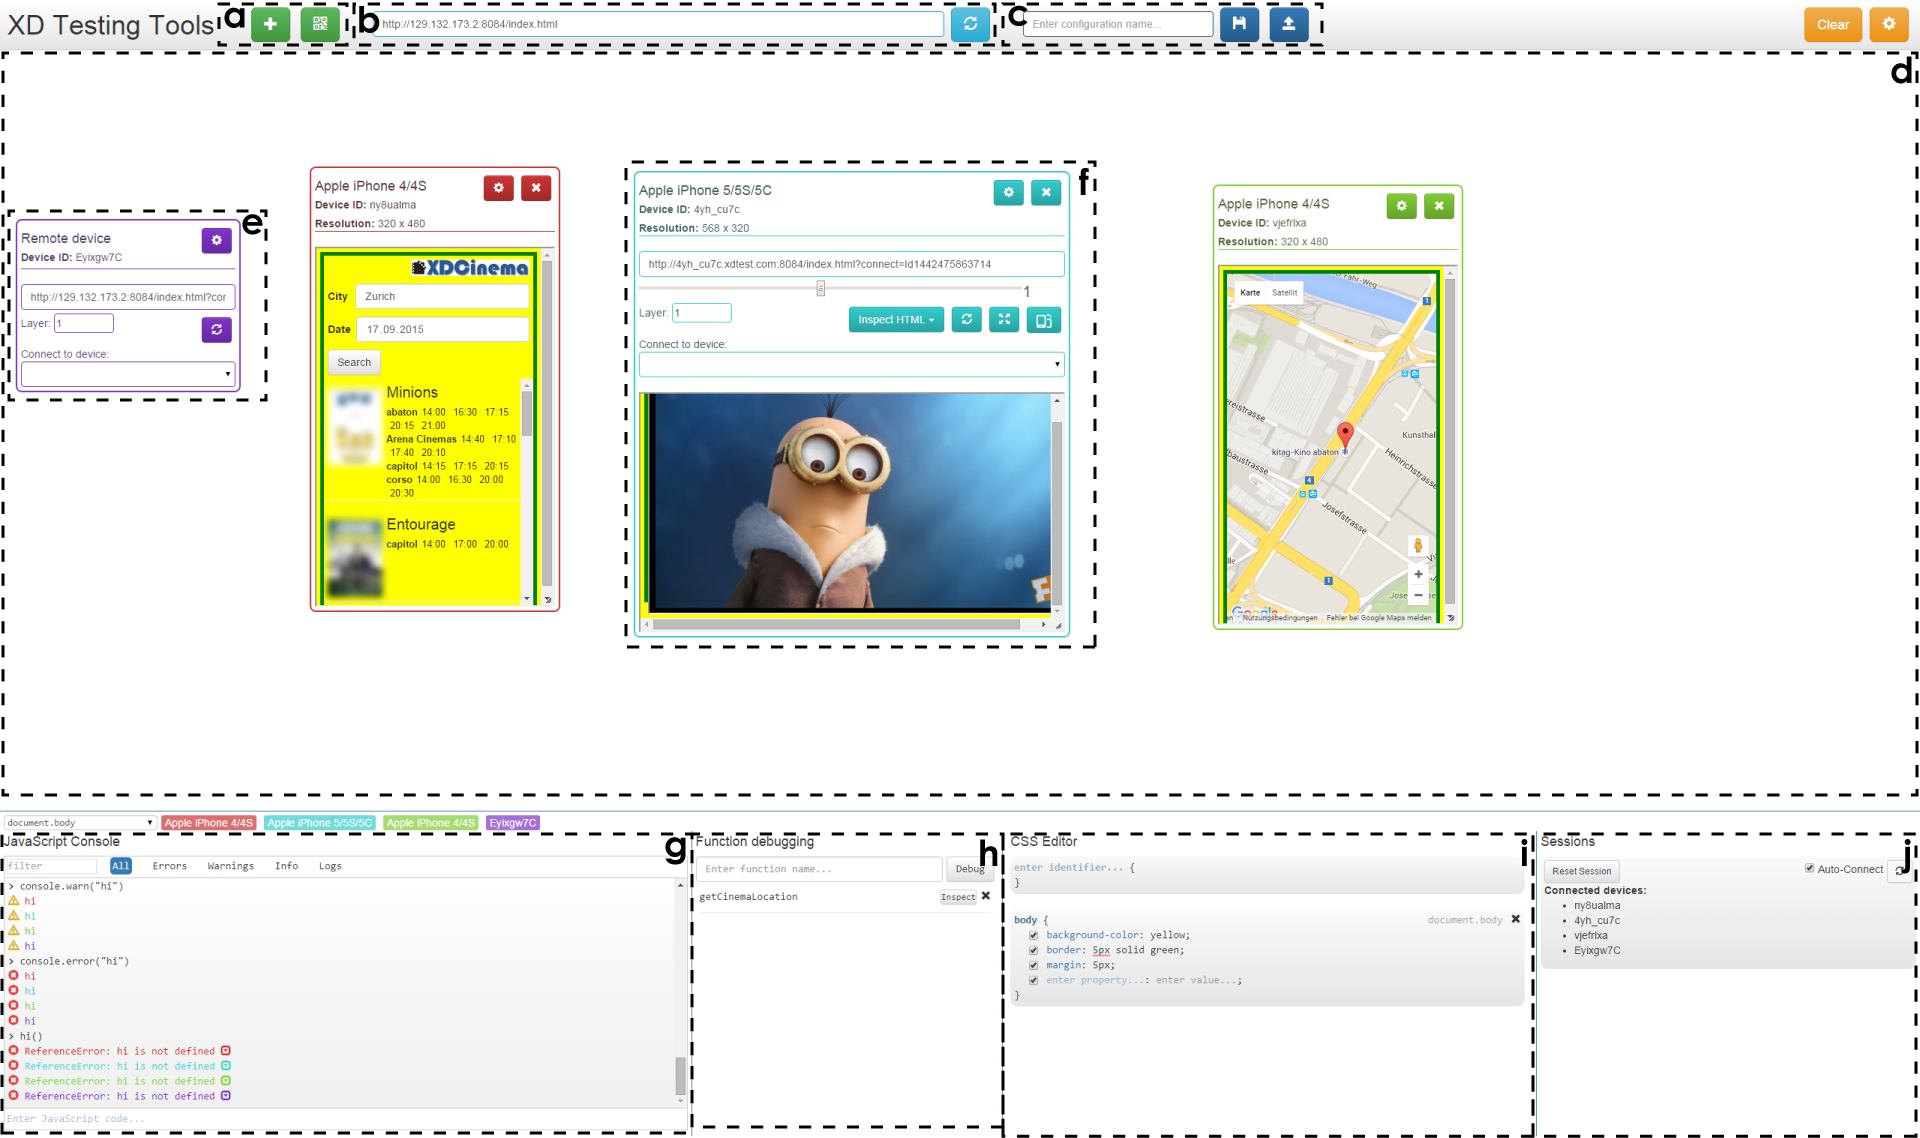
\includegraphics[width=1.0\textwidth]{images/screenshots/complete_3.png}
	\caption[Screenshot: Complete Interface]{The complete interface (without record and replay)}
	\label{fig:complete}
\end{figure}

The individual features of XDTools are labeled in the screenshot:
\begin{itemize}
	\item [a)] Buttons for adding emulated devices and showing the QR code for connecting real devices.
	\item [b)] Input field for loading a URL on all devices and button to refresh all devices.
	\item [c)] Loading and saving device configurations.
	\item [d)] Area where the devices can be positioned.
	\item [e)] Proxy of a connected real device.
	\item [f)] An emulated device.
	\item [g)] The shared JavaScript console.
	\item [h)] Function debugging.
	\item [i)] The shared CSS editor.
	\item [j)] Session management.
\end{itemize}

Figure~\ref{fig:complete_remote} shows a picture of the remote device that is connected to XDTools in the screenshot shown above.

\begin{figure}[H]
  \centering
    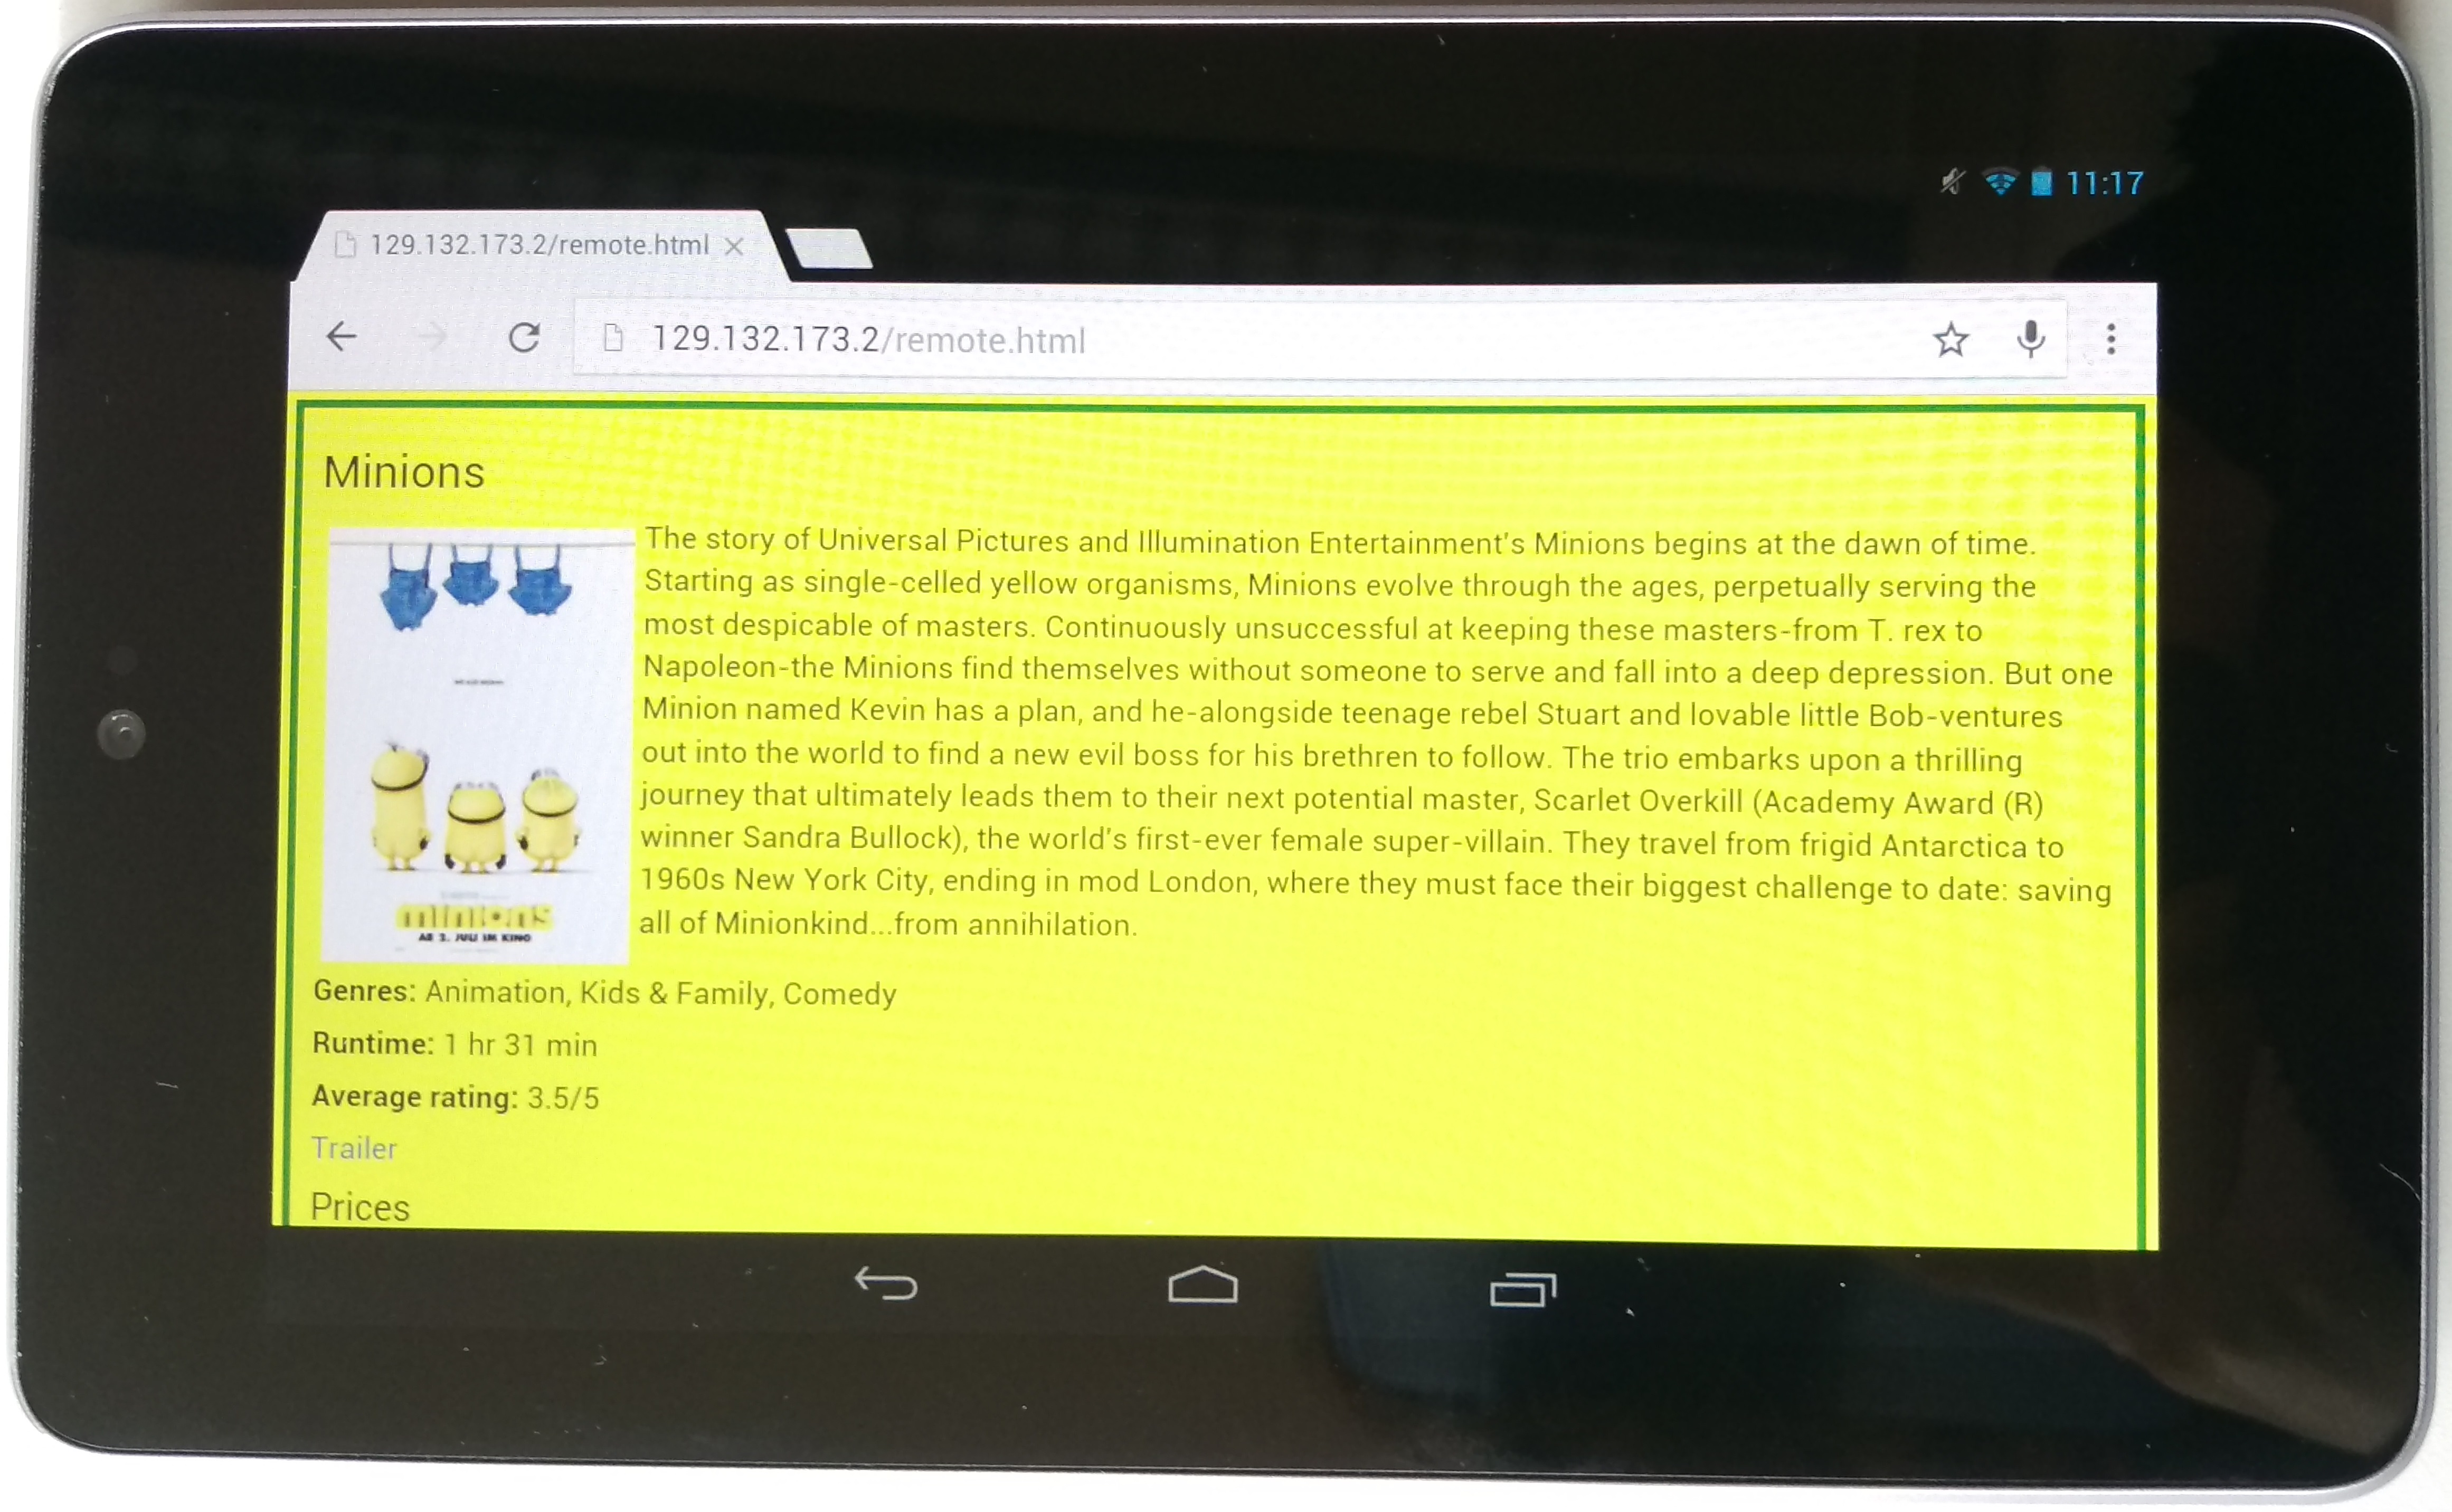
\includegraphics[width=1.0\textwidth]{images/screenshots/remote_device.jpg}
	\caption[Screenshot: Remote Device]{The connected remote device}
	\label{fig:complete_remote}
\end{figure}

XDTools also provides some options for disabling individual features, such as the shared JavaScript console. If a feature is disabled, the respective interface component is simply hidden. The options also show all stored custom devices, device configurations and event sequences and allow the developer to delete any of them. A screenshot of the options can be seen in Figure~\ref{fig:options}.

\begin{figure}[H]
  \centering
    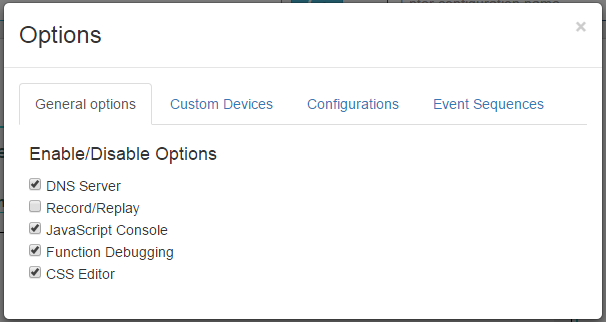
\includegraphics[width=0.9\textwidth]{images/screenshots/options.png}
	\caption[Screenshot: Options]{Options of our main application}
	\label{fig:options}
\end{figure}

Devices can also be activated and deactivated. If a device is inactive, it is not included for the following features:
\begin{itemize}
	\item Shared JavaScript console
	\item Shared CSS editor
	\item Function debugging
\end{itemize}
All those features perform some interactions with the devices automatically, thus they should be deactivated for inactive devices. Other features like record and replay still include inactive devices because manual interaction is needed anyway before something happens with the device. Devices can be activated and deactivated by clicking on their name/ID that is displayed above the JavaScript console. When the device is active, the background of its name is in the color of the device, otherwise it is grey and the text color is in the color of the device. Figure~\ref{fig:active_inactive} illustrates the difference between active and inactive devices. The first device is inactive, the other two devices are active.

\begin{figure}[H]
  \centering
    
\includegraphics[width=0.8\textwidth]{images/screenshots/active_inactive.png}
	\caption[Screenshot: Active/inactive devices]{Active and inactive devices}
	\label{fig:active_inactive}
\end{figure}

\section{Emulation of Multiple Devices}

XDTools allows the developer to emulate multiple devices simultaneously. The developer can either select the emulated devices from a list of existing devices or create a custom device. The developer can create a custom device just for one-time use, or they can save it to the list of existing devices for later use. This allows developers to quickly extend the devices they have access to with new devices. Devices can be assigned to one of four categories:
\begin{itemize}
	\item Desktop devices: For simplicity, this category includes desktop PCs as well as laptops.
	\item Tablets
	\item Mobile phones
	\item Wearables
\end{itemize}
Although some devices may not easily be classified, e.g. 2-in-1 devices that can either be used as a tablet or laptop by just plugging in a keyboard, those categories give a rough overview of the different types of devices. This categorization of devices also makes it easier for developers to emulate different types of devices without having to know any exact device names. By just adding some devices from each category, the developer can make sure that a large range of devices is covered, as devices in the same category typically have similar properties such as screen size and input modalities. Our list of existing devices includes multiple devices from each of those categories. For the desktop devices, we just provide some typical resolutions of desktop PCs and laptops. The list for tablets and mobile phones includes most of the well-known devices in that area. The list of wearables so far only includes some smart watches, as most other wearables do not have access to a modern web browser (yet). Figure~\ref{fig:adding_emulated} shows the menu for adding emulated devices.

\begin{figure}[H]
  \centering
    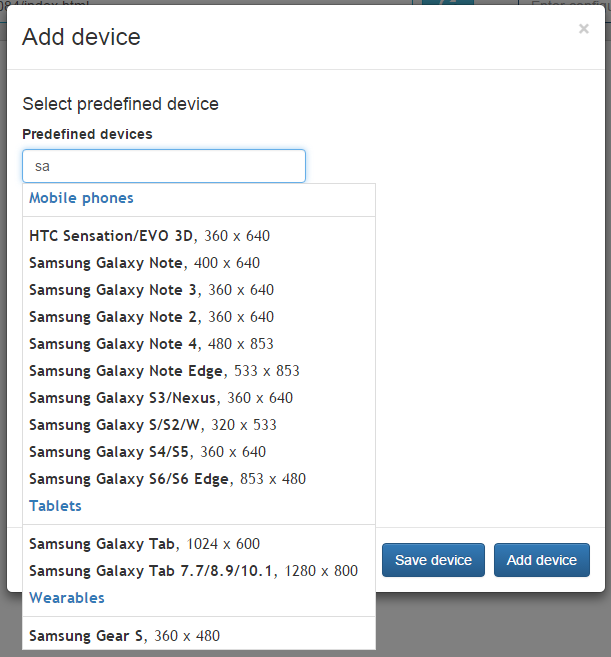
\includegraphics[width=0.8\textwidth]{images/screenshots/adding_device_predefined.png}
	\caption[Screenshot: Adding emulated devices]{Adding an emulated device}
	\label{fig:adding_emulated}
\end{figure}

Once the developer has created an emulated device (see Figure~\ref{fig:emulated_device}), they can move it to the desired location on the screen. Instead of ordering devices automatically, we chose to give the developer the freedom to choose how to place the emulated devices. This makes it easy to accurately simulate specific scenarios, e.g. a presentation room where two large screens are placed next to each other. To conquer the challenge of limited screen size, all emulated devices can be scaled up and down. Scaling a device does not change the resolution of the device and thus has no influence on the look of the application. This allows the developer to scale down an emulated device and have more space available for devices. If the developer has difficulties performing an interaction on a device because it is scaled down, they can just scale it up again. However, dynamically changing the resolution of an emulated device is also possible. Thus, the developer can continuously increase or decrease the resolution of the device to immediately see what the application looks with different resolutions. Finally, the developer can also change the layer of the device. Changing the layer of a device essentially moves the device to the front or back, thus devices can overlap each other and the developer can move the device that they want to use to the front.

\begin{figure}[H]
  \centering
    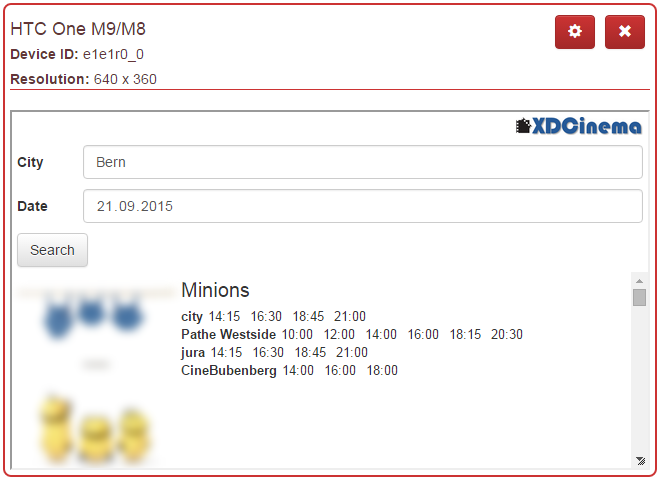
\includegraphics[width=0.8\textwidth]{images/screenshots/emulated_device_3.png}
	\caption[Screenshot: Emulated device]{An emulated device}
	\label{fig:emulated_device}
\end{figure}

Apart from its unique ID, each device also has a unique color. The border of the emulated device is colored with this color and the color is used in multiple other places for identifying the device. The devices also have a settings menu. In the settings menu, the developer can configure the following things:
\begin{itemize}
	\item The URL of the device.
	\item The scaling of the device.
	\item The orientation of the device.
	\item The layer of the device. 
	\item The device can be refreshed.
	\item The developer can inspect the HTML of the device.
	\item The developer can connect the device to another device by choosing it from a dropdown menu.
\end{itemize}
The device's settings are not constantly used by the developer and showing them at all times would occupy valuable screen space. Thus, the setting menu can be extended and collapsed by clicking a button. An example of a settings menu can be seen in Figure~\ref{fig:settings_menu}. 

\begin{figure}[H]
  \centering
    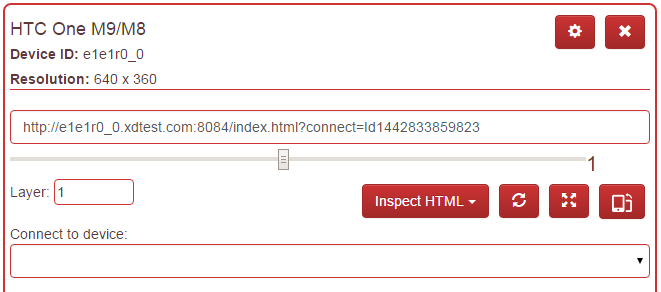
\includegraphics[width=0.8\textwidth]{images/screenshots/settings_menu_2.png}
	\caption[Screenshot: Settings menu emulated device]{Settings menu of an emulated device}
	\label{fig:settings_menu}
\end{figure}

Finally, XDTools also includes a mechanism that prevents the sharing of local resources between emulated devices.
 
\section{Easy Integration of Real and Emulated Devices}

QR codes have become increasingly popular over the last few years and almost all devices nowadays are equipped with at least one camera. Thus, XDTools includes a QR code that can be displayed and scanned by developers to connect a real device to XDTools. As a fallback mechanisms, devices can also be connected by typing a URL in the browser of the device. This makes it easy and efficient to connect a large number of real devices to XDTools. When the URL is opened, the device loads the application under test. The real devices only show the application under test and no interface elements. The developer can use the application on the real device, but everything relating to testing and debugging is coordinated through the developer's machine. Each connected real device is represented by a proxy within XDTools. The proxy of the real device also contains a settings menu similar to the one of an emulated device. However, the settings menu is missing a few things compared to emulated devices:
\begin{itemize}
	\item Scaling of the device: There is no need to scale real devices, as no \lstinline|iframe| is shown in the main application.
	\item Switching orientation: The orientation of a real device can be switched on the real device itself by simply rotating the real device.
	\item Inspecting the HTML: The developer's machine has no access to the HTML of the real device, thus it cannot be inspected.
\end{itemize}
Figure~\ref{fig:settings_menu_remote} shows the settings menu of a remote device. The settings menu only contains interface elements for setting the URL of the device, refreshing the application under test, changing the layer of the device and connecting the device to other devices.

\begin{figure}[H]
  \centering
    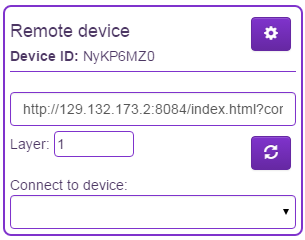
\includegraphics[width=0.5\textwidth]{images/screenshots/remote_device.png}
	\caption[Screenshot: Settings menu remote device]{Settings menu of a remote device}
	\label{fig:settings_menu_remote}
\end{figure}

The proxy of the real device can be moved around just like the emulated devices and its settings menu can also be collapsed and extended. Furthermore, each real device also has a unique ID and color for easy identification.

The developer can use emulated devices alongside real devices. Thus, XDTools allows the developer to test their application on only emulated devices, only real devices, or both at the same time. This flexibility makes it easy to test a large number of different scenarios.

\section{Easy Switching of Device Configurations}

XDTools allows the developer to create a device configuration, save it for later, and then re-use it. A device configuration consists of the following information:
\begin{itemize}
	\item The number of emulated devices.
	\item The types of the devices.
	\item The position and scaling of the devices.
\end{itemize}
The developer can easily re-use device configurations without much effort and switch between different device configurations efficiently. Thus, testing a cross-device application in many different device scenarios can be done without much effort. A user can just load one device configuration, try out the application and switch to the next device configuration if everything works as expected. The developer can also create a device configuration where only the static devices are saved in the configuration, e.g. in the example mentioned above, the developer could create a device scenario where only the big screens are already configured and then dynamically add some mobile devices to create a more realistic scenario.

For saving device configurations, the developer can type the name of a device configuration into an input field and then either click a save button to save the current device configuration under that name or click a load button to load a device configuration with that name (if it exists). Autocomplete is used for providing suggestions for existing device configurations that could be loaded (see Figure~\ref{fig:session_management}). 

\begin{figure}[H]
  \centering
    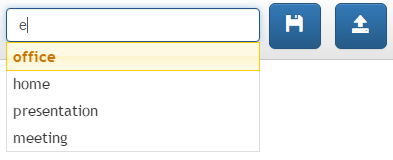
\includegraphics[width=0.6\textwidth]{images/screenshots/session_management_2.png}
	\caption[Screenshot: Saving/Loading device configurations]{Saving/Loading Device Configurations}
	\label{fig:session_management}
\end{figure}

\section{Integration with Debugging Tools}

For tighter integration with the browser's debugging tools, we included some popular tools that are already well-known from the debugging tools.

\subsection{Shared JavaScript Console}

XDTools includes a JavaScript console that is shared between all emulated and real devices. Each emulated and real device forwards all logging messages to the console. The console then aggregates all console outputs. Each message is displayed in the color of the device that it was sent from. This color-coding makes it trivial to identify the device a message originated from. Apart from forwarding logging messages, we also forward JavaScript errors. Whenever a JavaScript error occurs, the JavaScript error message is sent to the console, together with the stack trace if available. When a JavaScript error with stack trace is received by the console, the stack trace is split into multiple lines where each line represents one entry of the stack trace. By default, the developer only sees the error message itself without the stack trace. By clicking on a down-arrow button next to the error message, the developer can extend and collapse the stack trace. Figure~\ref{fig:stack_trace} shows what such a stack trace looks like in our JavaScript console.

\begin{figure}[H]
  \centering
    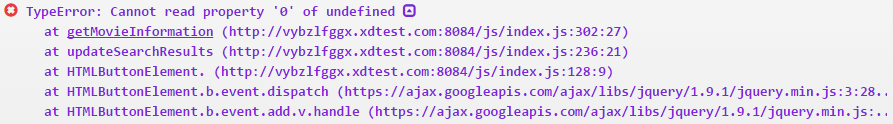
\includegraphics[width=1.0\textwidth]{images/screenshots/stack_trace_4.png}
	\caption[Screenshot: Stack trace]{Stack trace}
	\label{fig:stack_trace}
\end{figure}

For easier identification of the type of a message, all messages are assigned to one of four categories:
\begin{itemize}
	\item Warnings: This includes all warning logging messages.
	\item Errors: This includes all error logging messages and JavaScript errors.
	\item Info: This includes all info logging messages.
	\item Log: This includes all other types of messages.
\end{itemize}
Depending on the type of message, a different symbol is used in front of the message when it is displayed in the shared JavaScript console. This makes it easy to see if a message is an error or just a simple logging message.

The large number of messages that are displayed in the console due to the aggregation of many devices makes it a key requirement that there are some ways of filtering messages. The messages in the console can either be filtered by the type of message, e.g. show only all error messages, or by text. If the console messages are filtered by text, all messages that do not contain the text to filter by anywhere are hidden. If the filter is removed, the hidden messages are shown again. If a device is deactivated, it does not forward any messages or errors anymore and all existing messages are filtered out until the device is activated again. 

Our console also allows sending commands to multiple devices. If the developer wants to send a command to the devices, they can type the command into an input field below the console and press the enter key. The developer can either send the command to all devices or they can deactivate some devices and only send the message to a subset of devices. Being able to send a command only to a subset of devices is important in a cross-device setting because some commands might only make sense on some devices and executing them on all devices could lead to potential errors or a decrease in performance. The return values of commands are also displayed in the console, again color-coded to match the device they came from. Thus, otherwise complicated tasks like checking the value of a global variable become trivial. Our custom console works exactly the same for emulated as well as real devices. This aggregation of console outputs from both emulated and real devices at least partially eliminates the need for remote debugging.

The shared JavaScript console also has a history function similar to the console in Chrome DevTools. By using the arrow keys, the developer can navigate through the history and call previous commands again.

The screenshot in Figure~\ref{fig:js_console} shows the shared JavaScript console including a few examples of how to use it. First, the developer tries to call a function on all devices but makes a typo. Because the function with the typo in the name does not exist, an error message is displayed by all devices. The developer then notices the typo, types the correct function and sees the return values of the function (the coordinates of a cinema). Finally, the developer wants to see which roles have been assigned to the devices. They type the name of the variable that contains the roles and the value of this variable on all devices is shown in the console.

\begin{figure}[H]
  \centering
    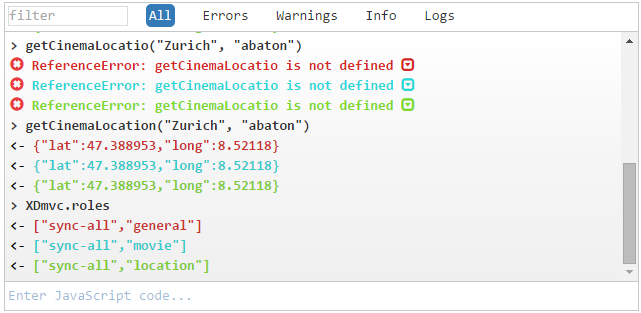
\includegraphics[width=1.0\textwidth]{images/screenshots/js_console_3.png}
	\caption[Screenshot: JavaScript console]{Shared JavaScript console}
	\label{fig:js_console}
\end{figure}

\subsection{Function Debugging and Inspection}

Function debugging allows developers to debug a function on all emulated devices or a subset of emulated devices without having to add breakpoints to each device individually.

In an area at the bottom of the interface of XDTools, the developer has access to an input field where they can type the name of the function they want to debug.  Below the input field, the list of functions that are currently debugged is shown. Whenever one of the debugged functions is called on any device, the debugger pauses at the beginning of the function and the developer can perform their debugging actions. The device on which the function was called is highlighted until the function call returns. This makes it easy to identify the device that is currently being debugged.

Figure~\ref{fig:function_debugging_complete} shows a screenshot while a function is being debugged. In the screenshot, the highlighted device, the Chrome DevTools with the debugged function and the list of debugged functions can be seen.

\begin{figure}[H]
  \centering
    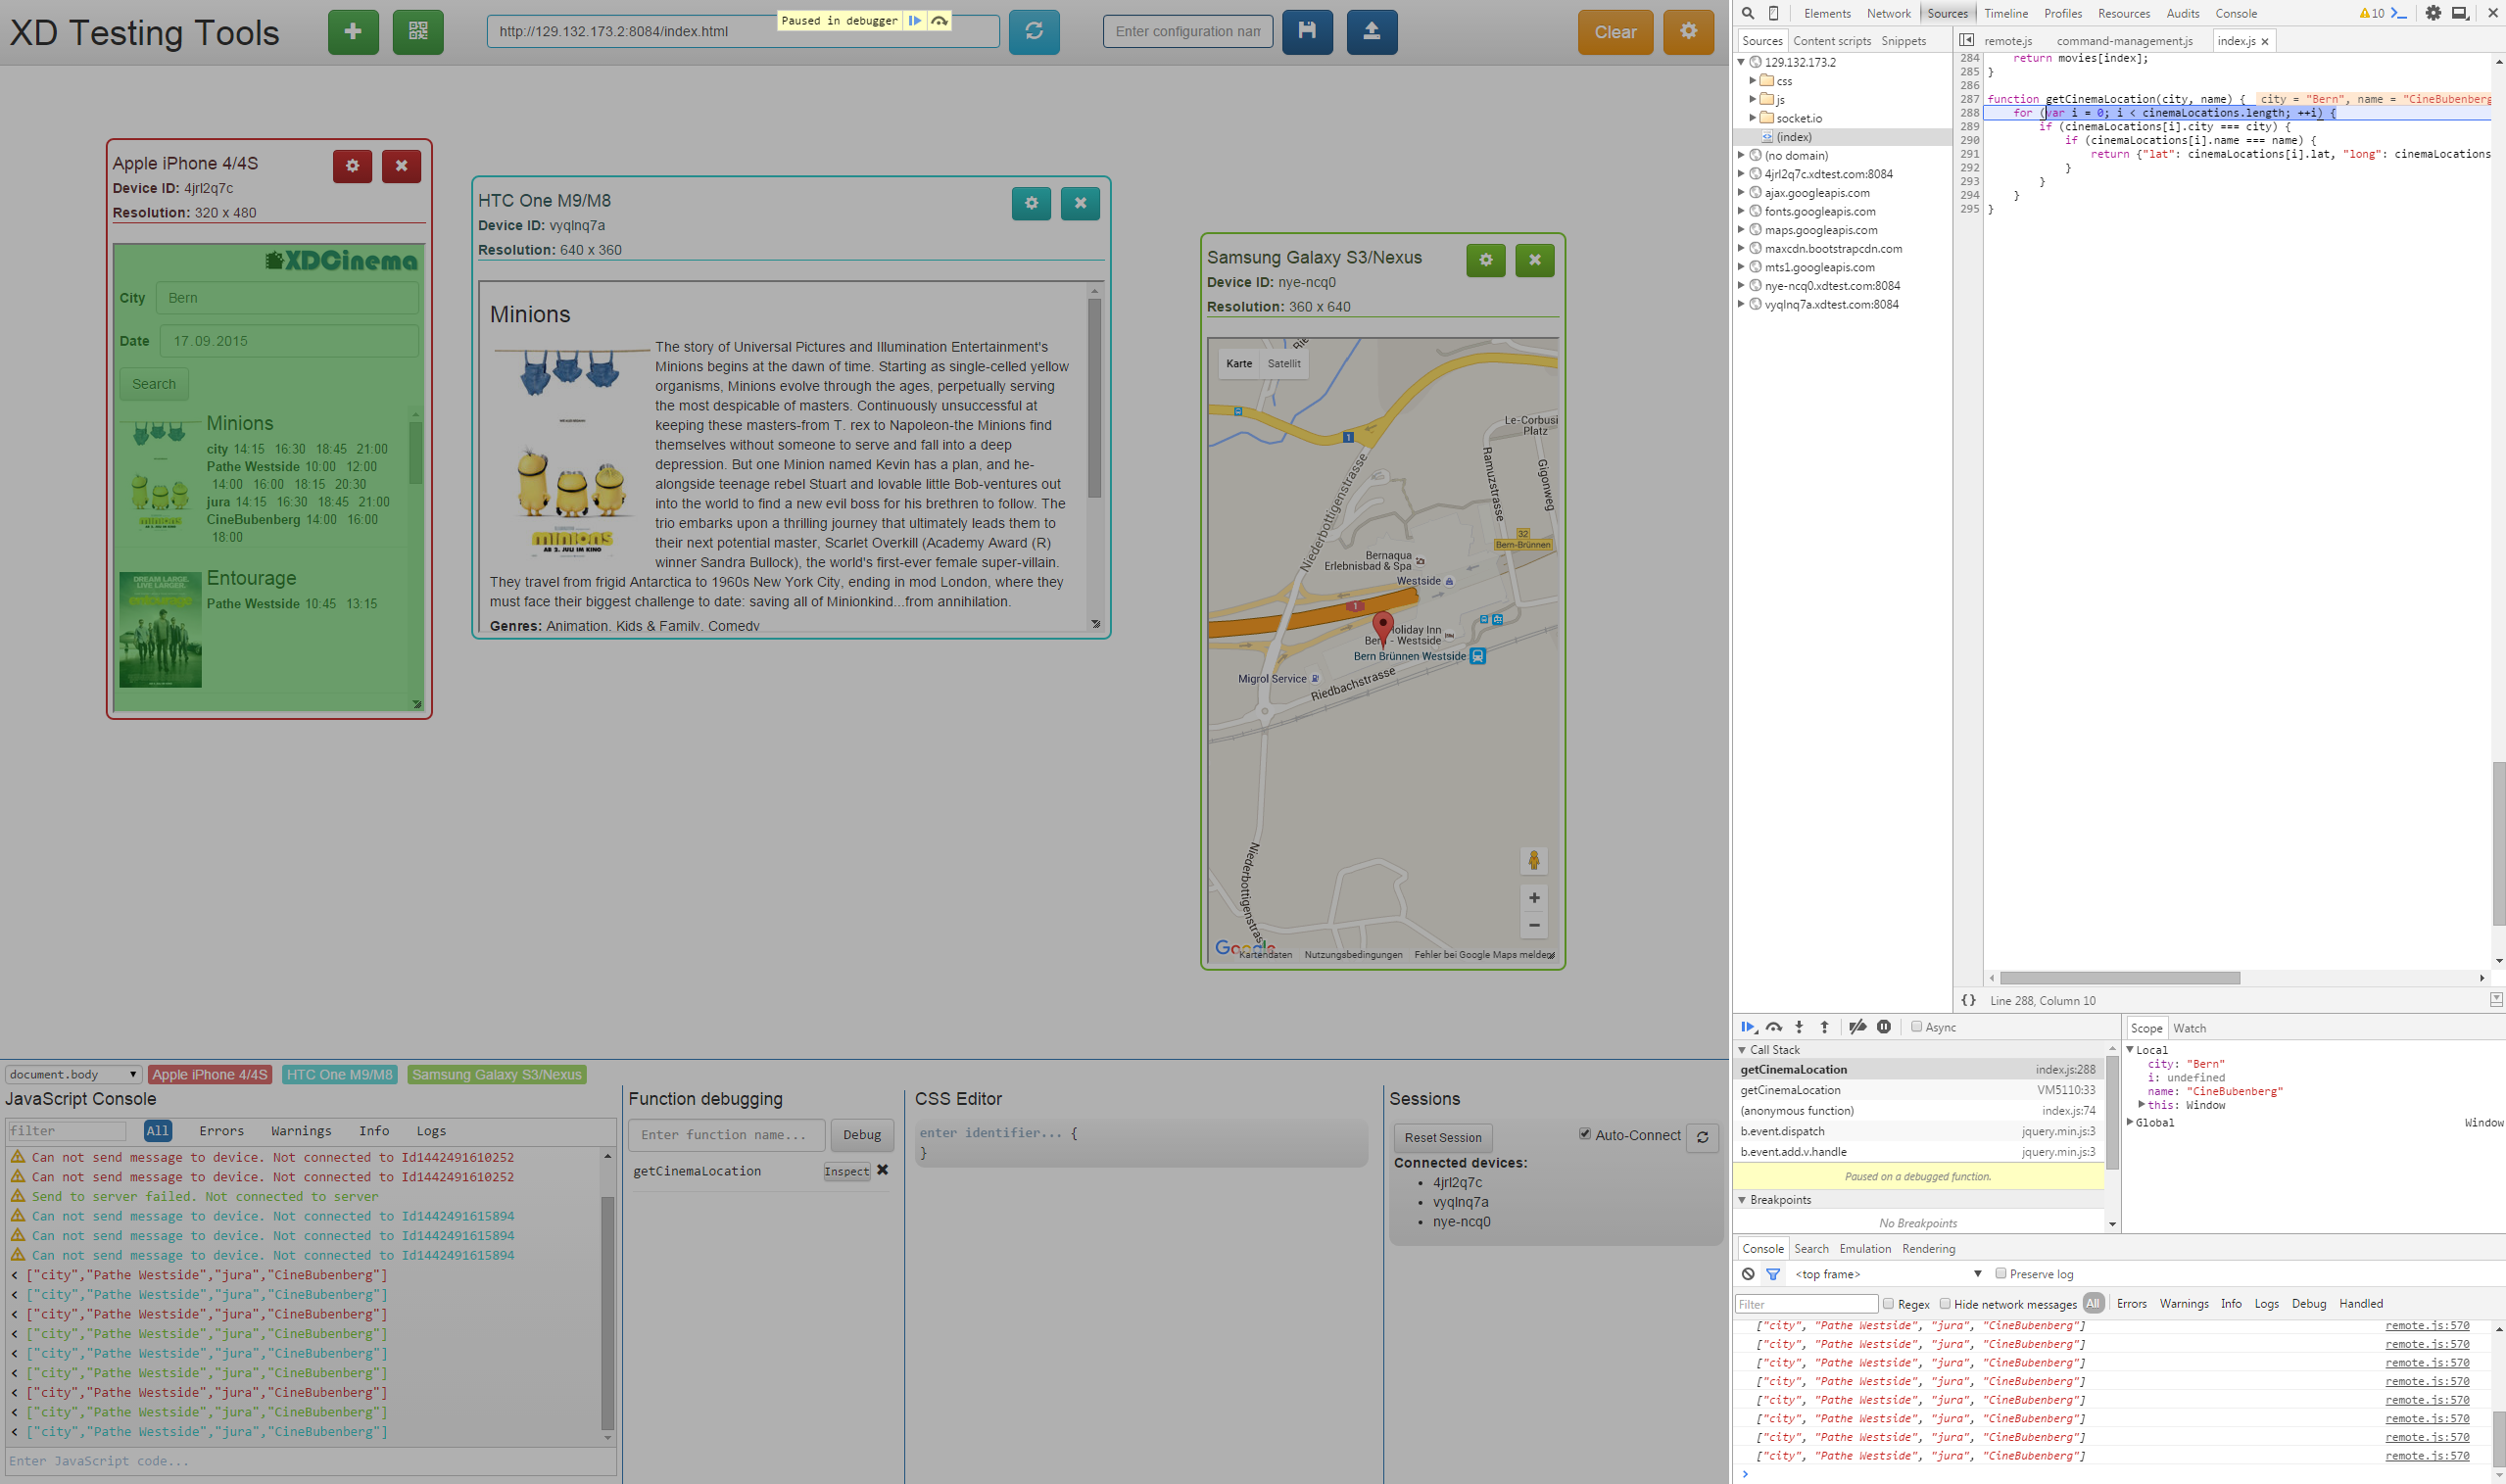
\includegraphics[width=1.0\textwidth]{images/screenshots/function_debugging_complete.png}
	\caption[Screenshot: Function debugging]{The complete interface while debugging a function}
	\label{fig:function_debugging_complete}
\end{figure}

If the developer is done debugging a function, they can remove it from the list of debugged functions.

The developer can also just inspect the function without it being called by clicking on a button next to the function name in the list of debugged functions. If this button is clicked, an emulated device is picked at random and the source code of the function is opened on this device. 

Unfortunately, function debugging only works on emulated devices. Chrome's DevTools do not have access to the JavaScript code of a connected real device, thus debugging the function using the DevTools is impossible.

\subsection{HTML Inspection}

XDTools allows the developer to directly jump into the HTML of an emulated device. Inside the settings menu of each emulated device, a button can be clicked to inspect the HTML of the device. Clicking this button opens the \lstinline|body| element of the device in the Chrome DevTools. 

HTML inspection is only available on emulated devices for the same reasons that we already mentioned before.

\subsection{Shared CSS Editor}

XDTools also includes a custom CSS editor. The CSS editor is designed to feel similar to the CSS editors typically provided by browsers. Thus, the developer can specify a selector and then add some rules that are applied to HTML elements that match the selector. The CSS rules are applied to all active devices, including both real and emulated devices. All CSS rules can be deactivated and activated again, edited, or removed completely. This allows the developer to quickly change the CSS of multiple devices and immediately see the result on all those devices. This is considerably less effort than adding rules to all devices individually or editing the CSS file, saving it and reloading all devices multiple times.

The CSS editor also has some autocomplete functionality: If the developer starts typing the name of a property, the property is automatically completed using the first CSS property name that matches the text typed by the developer (see Figure~\ref{fig:css_autocomplete}).

\begin{figure}[H]
  \centering
    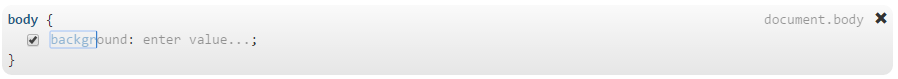
\includegraphics[width=1.0\textwidth]{images/screenshots/css_autocomplete.png}
	\caption[Screenshot: CSS editor autocomplete]{Autocomplete in the CSS editor}
	\label{fig:css_autocomplete}
\end{figure}

Figure~\ref{fig:css_editor} shows a screenshot of the CSS editor in action. In this screenshot, some CSS rules are added to the \lstinline|body| element of all devices.

\begin{figure}[H]
  \centering
    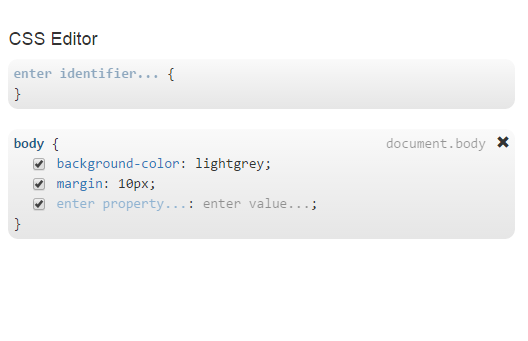
\includegraphics[width=1.0\textwidth]{images/screenshots/css_editor.png}
	\caption[Screenshot: CSS editor]{Shared CSS Editor}
	\label{fig:css_editor}
\end{figure}

In Figure~\ref{fig:css_applied}, the effects of the CSS shown in the screenshot above are shown. 

\begin{figure}[H]
  \centering
    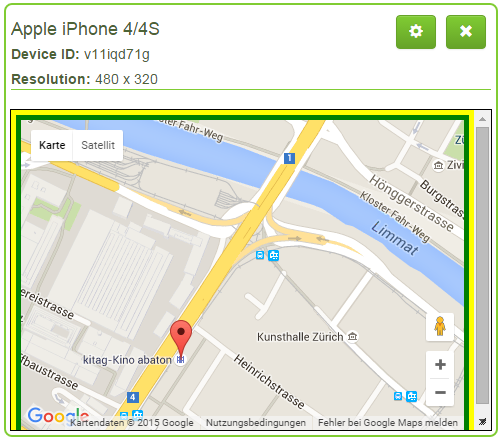
\includegraphics[width=0.5\textwidth]{images/screenshots/emulated_device_4.png}
	\caption[Screenshot: CSS effects]{CSS applied to emulated device}
	\label{fig:css_applied}
\end{figure}

\section{Automatic Connection Management}

The devices in XDTools can either be connected automatically or manually. Each set of connected devices represents a session. For each session, a checkbox allows the developer to toggle on or off auto-connect. When the first device is created or connected, auto-connect is turned on by default. If auto-connect is on, all newly created and connected devices will automatically be connected to that session. Thus, if the developer simply adds or connects a number of devices, they will automatically all be connected. If the developer wants to have multiple sessions, they can turn off auto-connect and then add more devices. Each device also has a drop-down menu in its settings menu for manually connecting to other devices. 

All current sessions are displayed at the bottom of the page of our application. Each session displays all connected devices (see Figure~\ref{fig:sessions}). The developer can also refresh all devices in a session and reset a session. Resetting a session assigns new IDs to all devices and thus erases the data of the devices. 

\begin{figure}[H]
  \centering
    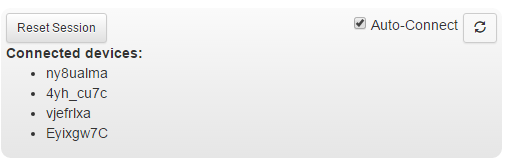
\includegraphics[width=0.6\textwidth]{images/screenshots/session_management.png}
	\caption[Screenshot: Session]{A device session}
	\label{fig:sessions}
\end{figure}

So far, automatic connection is only possible for applications that connect via URL. However, the URL required for connecting depends on the application. XDTools provides a custom connection function that can be adjusted by the developer such that it returns the appropriate URL.

\section{Coordinated Record and Replay}

XDTools allows the developer to record a sequence of interactions and replay them. Recording can be started on one device at any time. Once recording has started, the developer can perform the desired interactions on the device. After finishing recording, the interactions can be replayed on the same device, moved to other devices, or saved for later.  Furthermore, event sequences can be cut into multiple parts. The timing of the replays can be configured arbitrarily by dragging and dropping event sequences. This allows the developer to configure replays in many different ways: They can be executed in parallel, one after another, or anything in-between. The replays can then be started on all devices simultaneously r on one device at a time. This makes it easy to simulate multiple users and devices in a cross-device environment. Since the events contained in an event sequence are performed by a real user, i.e. the developer, the timing of the individual events in an event sequence is very realistic.

After a device finishes recording, the event sequence is visualized (Figure~\ref{fig:record_replay}).

\begin{figure}[H]
  \centering
    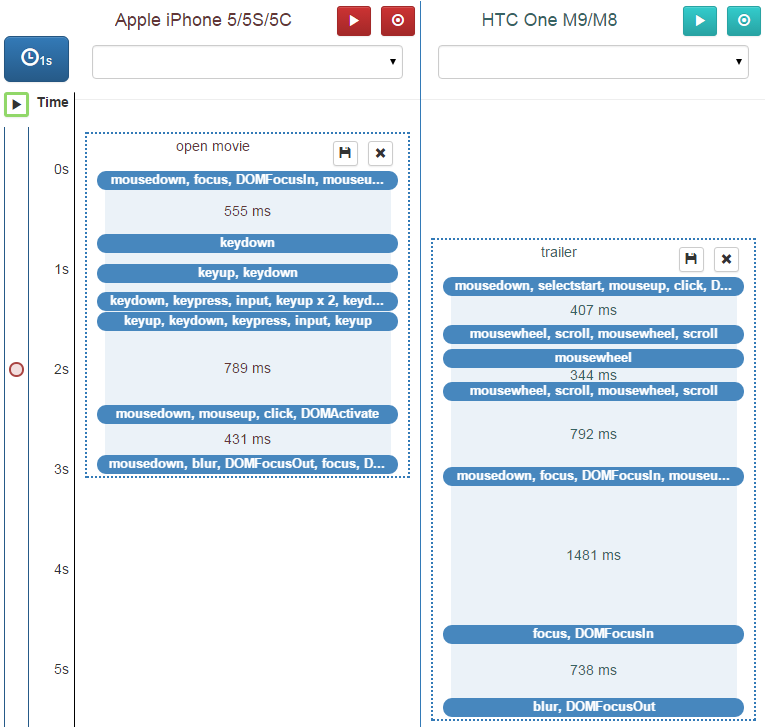
\includegraphics[width=1.0\textwidth]{images/screenshots/record_replay_2.png}
	\caption[Screenshot: Record and replay]{Record and Replay}
	\label{fig:record_replay}
\end{figure}

Furthermore, the developer can add breakpoints to the timing of the replay. Next to the event visualizations, a timeline is shown as well as a narrow empty column where the developer can click to add a breakpoint at a certain point in time. As soon as all events that occur before this point of time have been replayed, the replaying pauses and the developer can inspect the state of the devices. If a breakpoint is reached, the breakpoint that was reached is highlighted. After the developer chooses to continue, replaying is continued until the next breakpoint is reached. After the last breakpoint has been reached, the event replaying continues until all events have been replayed. The developer can also add breaks of one second between events to delay all following events. This allows the developer to spend some more time looking at the application before the replaying continues without having to set breakpoints. 